\documentclass[12pt,oneside]{book}
\usepackage[margin=1in]{geometry}
\usepackage{iftex}
\ifPDFTeX
  \usepackage[T1]{fontenc}
  \usepackage[utf8]{inputenc}
  \usepackage{lmodern}
\else
  \usepackage{fontspec}
  \setmainfont{Latin Modern Roman}
\fi
\usepackage{amsmath,amssymb,amsthm,mathtools}
\usepackage{longtable,booktabs}
\usepackage{enumitem}
\usepackage{setspace}
\usepackage{fancyhdr}
\usepackage{titlesec}
\usepackage[dvipsnames]{xcolor}
\usepackage{xurl}
\usepackage{textcomp}
\usepackage{hyperref}
\usepackage[nameinlink,noabbrev]{cleveref}
\usepackage[most]{tcolorbox}
\usepackage{microtype}
\usepackage{framed}
\usepackage{fancyvrb}
\usepackage{math-proofread-style}

\hypersetup{
  colorlinks=true,
  linkcolor=blue!50!black,
  citecolor=blue!50!black,
  urlcolor=blue!60!black,
  pdftitle={First Proof, Lakatos-Style},
  pdfauthor={Codex}
}

\Urlmuskip=0mu plus 1mu
\setcounter{tocdepth}{2}
\setcounter{secnumdepth}{3}
\setlength{\parskip}{0.2em}
\setlength{\parindent}{0pt}
\setlist[itemize]{itemsep=0.3em,topsep=0.3em}
\setlist[enumerate]{itemsep=0.3em,topsep=0.3em}
\setstretch{1.08}
\EnableMathProofColors

\providecommand{\tightlist}{}
\definecolor{shadecolor}{RGB}{248,248,248}
\DefineVerbatimEnvironment{Highlighting}{Verbatim}{commandchars=\\\{\}}
\newenvironment{Shaded}{\begin{snugshade}}{\end{snugshade}}
\providecommand{\NormalTok}[1]{#1}
\providecommand{\KeywordTok}[1]{#1}
\providecommand{\StringTok}[1]{#1}
\providecommand{\CommentTok}[1]{#1}
\providecommand{\FunctionTok}[1]{#1}
\providecommand{\VariableTok}[1]{#1}
\providecommand{\ControlFlowTok}[1]{#1}
\providecommand{\OperatorTok}[1]{#1}
\providecommand{\BuiltInTok}[1]{#1}
\providecommand{\DecValTok}[1]{#1}
\providecommand{\FloatTok}[1]{#1}
\providecommand{\ConstantTok}[1]{#1}
\providecommand{\ErrorTok}[1]{#1}
\providecommand{\PreprocessorTok}[1]{#1}
\providecommand{\ExtensionTok}[1]{#1}
\providecommand{\SpecialCharTok}[1]{#1}
\providecommand{\CharTok}[1]{#1}
\providecommand{\ImportTok}[1]{#1}
\providecommand{\DocumentationTok}[1]{#1}
\providecommand{\AnnotationTok}[1]{#1}
\providecommand{\AttributeTok}[1]{#1}
\providecommand{\InformationTok}[1]{#1}
\providecommand{\WarningTok}[1]{#1}
%
\ifPDFTeX
  \DeclareUnicodeCharacter{2218}{\ensuremath{\circ}}
  \DeclareUnicodeCharacter{2297}{\ensuremath{\otimes}}
  \DeclareUnicodeCharacter{2713}{\ensuremath{\checkmark}}
  \DeclareUnicodeCharacter{2202}{\ensuremath{\partial}}
  \DeclareUnicodeCharacter{2245}{\ensuremath{\cong}}
  \DeclareUnicodeCharacter{2227}{\ensuremath{\wedge}}
  \DeclareUnicodeCharacter{2295}{\ensuremath{\oplus}}
  \DeclareUnicodeCharacter{2229}{\ensuremath{\cap}}
  \DeclareUnicodeCharacter{220E}{\ensuremath{\square}}
  \DeclareUnicodeCharacter{2260}{\ensuremath{\neq}}
  \DeclareUnicodeCharacter{2261}{\ensuremath{\equiv}}
  \DeclareUnicodeCharacter{2264}{\ensuremath{\le}}
  \DeclareUnicodeCharacter{2265}{\ensuremath{\ge}}
  \DeclareUnicodeCharacter{2282}{\ensuremath{\subset}}
  \DeclareUnicodeCharacter{2286}{\ensuremath{\subseteq}}
  \DeclareUnicodeCharacter{222A}{\ensuremath{\cup}}
  \DeclareUnicodeCharacter{2208}{\ensuremath{\in}}
  \DeclareUnicodeCharacter{2192}{\ensuremath{\to}}
  \DeclareUnicodeCharacter{00B7}{\ensuremath{\cdot}}
  \DeclareUnicodeCharacter{229E}{\ensuremath{\boxplus}}
  \DeclareUnicodeCharacter{00D7}{\ensuremath{\times}}
  \DeclareUnicodeCharacter{03B8}{\ensuremath{\theta}}
  \DeclareUnicodeCharacter{03BD}{\ensuremath{\nu}}
  \DeclareUnicodeCharacter{03C0}{\ensuremath{\pi}}
  \DeclareUnicodeCharacter{03C1}{\ensuremath{\rho}}
  \DeclareUnicodeCharacter{0393}{\ensuremath{\Gamma}}
  \DeclareUnicodeCharacter{221A}{\ensuremath{\sqrt}}
  \DeclareUnicodeCharacter{00B1}{\ensuremath{\pm}}
  \DeclareUnicodeCharacter{00B9}{\textsuperscript{1}}
  \DeclareUnicodeCharacter{00B2}{\textsuperscript{2}}
  \DeclareUnicodeCharacter{2081}{\textsubscript{1}}
  \DeclareUnicodeCharacter{2083}{\textsubscript{3}}
  \DeclareUnicodeCharacter{2088}{\textsubscript{8}}
\fi

\newcommand{\gapnote}[1]{%
  \par\medskip
  \noindent\fcolorbox{red!60!black}{red!4}{%
    \parbox{0.96\linewidth}{\textbf{Open Gap / Conditional Step.} #1}%
  }%
  \par\medskip
}
\newcommand{\statusnote}[1]{%
  \par\medskip
  \noindent\fcolorbox{green!50!black}{green!4}{%
    \parbox{0.96\linewidth}{\textbf{Status Note.} #1}%
  }%
  \par\medskip
}
% --- Dialogue boxes for Part III ---
\newtcolorbox{joebox}[1][]{%
  colback=orange!4, colframe=orange!50!black,
  fonttitle=\bfseries\sffamily\small,
  title={Joe}, #1,
  left=6pt, right=6pt, top=4pt, bottom=4pt,
  boxrule=0.5pt, arc=2pt,
  before skip=6pt, after skip=2pt
}
\newtcolorbox{claudebox}[1][]{%
  colback=blue!3, colframe=blue!40!black,
  fonttitle=\bfseries\sffamily\small,
  title={Claude}, #1,
  left=6pt, right=6pt, top=4pt, bottom=4pt,
  boxrule=0.5pt, arc=2pt,
  before skip=2pt, after skip=2pt
}
\newtcolorbox{codexbox}[1][]{%
  colback=green!3, colframe=green!40!black,
  fonttitle=\bfseries\sffamily\small,
  title={Codex}, #1,
  left=6pt, right=6pt, top=4pt, bottom=4pt,
  boxrule=0.5pt, arc=2pt,
  before skip=2pt, after skip=2pt
}
\newcommand{\pivot}[1]{%
  \par\smallskip
  \noindent{\small\sffamily\color{black!60}%
    \textbf{Pivot:}\space #1}%
  \par\smallskip
}
% --- End dialogue boxes ---

\newcommand{\includeannotated}[1]{%
  \begingroup
  \let\origsection\section
  \let\origsubsection\subsection
  \let\origsubsubsection\subsubsection
  \let\section\chapter
  \let\subsection\origsection
  \let\subsubsection\origsubsection
  \input{#1}
  \endgroup
}
\newcommand{\includefull}[1]{%
  \begingroup
  \let\origsection\section
  \let\origsubsection\subsection
  \let\origsubsubsection\subsubsection
  \let\section\chapter
  \let\subsection\origsection
  \let\subsubsection\origsubsection
  \input{#1}
  \endgroup
}

\titleformat{\chapter}[display]
  {\bfseries\Large}
  {\filright\large\chaptername\ \thechapter}
  {0.6em}
  {\filright}
\titlespacing*{\chapter}{0pt}{-6pt}{18pt}

\pagestyle{fancy}
\fancyhf{}
\fancyhead[LE,RO]{\thepage}
\fancyhead[LO]{\nouppercase{\rightmark}}
\fancyhead[RE]{\nouppercase{\leftmark}}
\renewcommand{\headrulewidth}{0.2pt}

\title{First Proof, Lakatos-Style}
\author{Claude$^{1}$, Codex$^{2}$, J.~Corneli$^{3}$\thanks{Supervisor} \\
\small $^{1}$Anthropic \quad $^{2}$OpenAI \quad $^{3}$Hyperreal Enterprises Ltd}
\date{February 12, 2026}

\begin{document}
\frontmatter
\begingroup
\renewcommand{\thefootnote}{\fnsymbol{footnote}}
\maketitle
\endgroup
\setcounter{footnote}{0}
\renewcommand{\thefootnote}{\arabic{footnote}}
\tableofcontents

\chapter*{Reader Guide}
This document is organized in three layers.

\begin{itemize}[leftmargin=1.5em]
\item \textbf{Part I (Annotated Overview):} short, citation-rich introductions for Problems 1--10, intended as navigational summaries.
\item \textbf{Part II (Full Proof Drafts):} expanded writeups imported from the solution files, suitable as the base for a longer manuscript (targeting roughly book-length exposition).
\item \textbf{Part III (Prompt Excerpts and Pivot Moments):} curated source excerpts (prompts and dispatch/history snippets) that document key decision points and proof-state transitions.
\end{itemize}

Problem 6 currently retains an explicit unresolved obligation in the project state. Problem 7 is treated in this manuscript revision as closed via the updated rotation-route theorem chain.
\chapter*{Introduction: The Making of the First-Proof Cycle}
\addcontentsline{toc}{chapter}{Introduction: The Making of the First-Proof Cycle}

\section*{Highlights}
\begin{itemize}[leftmargin=1.5em]
\item Dependency-graph representations of proofs enabled local gap isolation and targeted repair across all ten problems.
\item Node-level verification with predecessor/successor context improved calibration relative to whole-draft review.
\item Adversarial critic--responder iteration converted early overclaims into explicit closed, partial, or conditional outcomes.
\item Targeted computational stress tests constrained speculative branches, especially in the \(n=4\) branch of Problem~4.
\item Structured handoff memos preserved unresolved obligations as named, testable next steps rather than implicit deferrals.
\end{itemize}

\section*{Snapshot}
\begin{itemize}[leftmargin=1.5em]
\item Ten initial proof attempts drafted in under two hours.
\item Over two hundred commits across roughly 55~hours wall-clock (February 11--13, 2026), in addition to earlier infrastructure development.
\item A shift in framing over the course of the sprint: from an early ``all solved'' posture to a clearer partition into proved, conditional, and partial results.
\item A methodological lesson: wiring-diagram--based verification localized gaps and inconsistencies more effectively than plain narrative drafting.
\end{itemize}

\section*{Materials and Methods}
\begin{itemize}[leftmargin=1.5em]
\item \textbf{Model/runtime split.} Claude Max runs on a remote Linode host; Codex Pro runs on the local laptop workspace (\texttt{/home/joe/code/futon6}).
\item \textbf{Software/toolchain summary.} Computational checks used Python~3 scripts with NumPy/SciPy for numerical linear algebra and optimization, SymPy for symbolic algebra (resultants, Sturm sequences, Gr\"obner bases), mpmath for selected high-precision checks, PHCpack via \texttt{phcpy} for polynomial-system solving/certification in Problem~4 (Case~3c), and cvxpy for SDP-based sum-of-squares certificate attempts. Proof-structure analysis used wiring-diagram generators (nine scripts producing JSON and Mermaid flowcharts via the internal \texttt{thread\_performatives} module) and \texttt{validate-ct.py} for classical NER and scope extraction over PlanetMath entries. Pattern tagging and term spotting used Babashka (Clojure) scripts operating on EDN data formats. Document production used \LaTeX{} (\texttt{pdflatex}) with repository consistency-checking scripts (\texttt{check-latex-syntax-violations.py}, \texttt{check-ratchet-fixedw-typesetting.py}).
\item \textbf{Codex Pro token accounting (local, log-derived).} From \texttt{\~{}/.codex/sessions/*} telemetry (records where the event type is \emph{token\_count}), over the 50-hour window ending 2026-02-13 21:41 UTC (window start: 2026-02-11 19:41 UTC), there were 333 futon6-related Codex rollout traces out of 334 local rollout traces (99.7\%). Aggregated futon6 usage totals: total tokens 965{,}714{,}475; input tokens 961{,}719{,}044 (including cached input tokens 912{,}686{,}208, so non-cached input \(\approx 49{,}032{,}836\)); output tokens 3{,}995{,}431; reasoning-output tokens 2{,}072{,}289.
\item \textbf{Claude Max token accounting (Linode, log-derived).} From \texttt{\~{}/.claude/projects/*/} session files on the Linode host, 9 futon6-related Claude~Code sessions were identified (8 contributing within the 50-hour Codex-comparable window). Over the same 50-hour window ending 2026-02-13 21:41 UTC (window start: 2026-02-11 19:41 UTC), aggregated futon6 usage totals: total tokens 791{,}980{,}382; input tokens 789{,}643{,}774 (including cached-read input tokens 752{,}300{,}790, cache-creation input tokens 37{,}221{,}978, non-cached input \(\approx 121{,}006\)); output tokens 2{,}336{,}608. Model: \texttt{claude-opus-4-6} (7{,}754 assistant messages). Full-window totals (9~sessions, 2026-02-08 through 2026-02-13): total tokens 1{,}021{,}665{,}524; output tokens 2{,}798{,}074.
\end{itemize}

\section*{Introduction}
This monograph records both the mathematical results and the working process
behind a compressed, multi-agent proof cycle in \texttt{futon6}.\footnote{Source repository: \url{https://github.com/tothedarktowercame/futon6}} The project
began as infrastructure---knowledge ingestion, tagging, and wiring-diagram
metatheory---and then pivoted into a rapid proof sprint with iterative
critique and repair.

The working process turned out to resemble Lakatos's \emph{Proofs and
Refutations}~\cite{lakatos1976} more than we expected. In Lakatos's
dialogue, a conjecture is proposed, counterexamples surface, the conjecture
is patched, and the cycle repeats---with each iteration sharpening both the
theorem and the participants' understanding of the domain. Our sprint
followed the same rhythm, except that the interlocutors were a human
dispatcher, multiple Claude instances (provers), and Codex (critic and
research assistant). Conjectures were drafted quickly; adversarial review
surfaced overclaims and gaps; targeted repair narrowed the open obligations.
The wiring-diagram decomposition---which represents each proof as a typed
graph of claims and dependencies---served as the shared epistemic artefact
that Lakatos's blackboard served in his fictional classroom.

The title alludes to the sprint format: ten open problems attempted in
roughly 55~hours wall-clock, with the process documented alongside the results.
The Lakatosian connection runs through Pease et
al.~\cite{pease2017}, which formalised Lakatos's informal logic of
mathematical discovery as a dialogue game over argumentation structures,
implemented in a system capable of mixed-initiative human--AI collaboration.
That paper asked whether computers could participate in mathematical
reasoning the way humans do---through conjecture, critique, and reform.
The present work is, in a sense, a large-scale empirical answer: ten
problems attempted by AI agents under human supervision, with the
Lakatosian cycle running at machine speed.

This connection is not accidental. Corneli et al.~\cite{corneli2017}
developed a computational model of mathematical question-and-answer dialogues
grounded in Lakatos's framework, using Inference Anchoring Theory + Content
(IATC) to annotate MathOverflow threads with performative types
(assert, challenge, reform, clarify, etc.). The IATC vocabulary reappears in
this project's Stage~7 thread-wiring pipeline (see Part~III, Act~VI), where
StackExchange threads are parsed into wiring diagrams whose edges carry the
same performative labels. The earlier work on peer-produced mathematical
knowledge~\cite{corneli2013} established the empirical base: PlanetMath as a
community-maintained proof ecosystem, studied through the lens of paragogy
(peer-produced peer learning). The present sprint can be read as a
machine-accelerated instance of the same phenomenon: collaborative,
incremental proof construction with explicit argumentation structure.

The working notes reveal a consistent asymmetry: generation is fast;
trustworthy validation is slow. This is the same asymmetry Lakatos
identified in his classroom: conjectures are cheap, but understanding
\emph{why} a conjecture fails (or holds) is the real mathematical work.
In practice, the strongest leverage came from structured verification---tools
that made weaknesses visible early and locally.

\section*{Reader Guide}
This document is organized in five parts.

\begin{itemize}[leftmargin=1.5em]
\item \textbf{Part I (Annotated Overview):} short, citation-rich introductions for Problems 1--10, intended as navigational summaries.
\item \textbf{Part II (Full Proof Drafts):} expanded writeups imported from the solution files, suitable as the base for a longer manuscript (targeting roughly book-length exposition). Coloured boxes separate the proof proper from process annotations (dead paths, revisions, open obligations).
\item \textbf{Part III (Prompt Excerpts and Pivot Moments):} curated source excerpts (prompts and dispatch/history snippets) that document key decision points and proof-state transitions.
\item \textbf{Part IV (Proof Patterns):} a cross-problem analysis of strategy patterns---what worked (layer-switching, creative reduction, structural decomposition), what didn't (the TryHarder loop), and how a coaching intervention broke a stuck problem open.
\item \textbf{Part V (Color Plates):} syntax-coloured renderings of the proof files, produced by automated math-mode normalization.
\end{itemize}

\section*{Terminology}
\begin{description}[leftmargin=1.5em,style=nextline]
\item[AIF] Active Inference Framework---used here as a conceptual lens for agent roles, intervention points, and coordination state; a full AIF policy loop for proof search is proposed future work, not yet implemented in this sprint.
\item[BSS] Batson--Spielman--Srivastava spectral sparsification framework.
\item[IATC] Inference Anchoring Theory + Content---an annotation scheme for mathematical dialogues used here to type dialogue moves and content links within the AIF process model~\cite{corneli2017}.
\item[MSS] Marcus--Spielman--Srivastava interlacing families framework.
\item[PSD] Positive semi-definite (for matrices).
\end{description}

\section*{Current Status}
\noindent\textbf{Status legend.}
Each problem is tagged on two axes:
\textbf{Closed/Partial/Conditional} for mathematical status and
\textbf{Validation-complete/Partial validation} for QC-validation status.

\medskip
\noindent\textbf{Outcome summary.}
Problem~3 is closed for the scoped existence target and validation-complete;
Problem~5 is closed in a scope-limited form;
Problem~10 is conditional under stated assumptions;
Problems~4 and~6 are partial with explicit remaining obligations;
Problem~7 is provisionally closed mathematically (rotation route), with QC
review still active; and Problems~1,~2,~7,~8, and~9 are partial-validation at
node level due to unresolved verifier gaps.

\begin{itemize}[leftmargin=1.5em]
\item Problems 1, 2, 8, and 9 now have node-level validation artifacts.\footnote{Per-problem verifier outputs are tracked in \url{https://github.com/tothedarktowercame/futon6/tree/master/data/first-proof} under filenames matching \texttt{problem*-codex-results.jsonl}.} Each currently remains in \emph{partial validation} due to unresolved node-level gaps flagged by the verifier.
\item Problem 7 is treated as provisionally closed mathematically via the rotation route, while remaining in \emph{partial validation} at QC level pending independent ledger re-check and closure of verifier-flagged nodes.
\item Problem 3 now has a validation-complete existence path under the scoped criterion used here (current run: 2 verified, 7 plausible, 0 gaps). Uniqueness/irreducibility is treated as optional and out of scope for the core existence claim.
\item Problem 10 is conditional under explicitly stated assumptions, with explicit necessity counterexamples for assumption violations.
\item Problem 5 is solved in a scope-limited form for $F_O$-local connective spectra.
\item Problem 6 is partial: the $K_n$ case is proved ($c_0 = 1/3$), with one remaining technical gap in the general-graph argument (formal $\bar{d} < 1$ bound at $M_t \ne 0$).
\item Problem 4 is partial: proved analytically for $n \le 3$; the $n=4$ branch has strong computational support with one certification step still pending; higher $n$ remains open.
\item Cross-problem closure-vs-validation inventory.\footnote{\url{https://github.com/tothedarktowercame/futon6/blob/master/data/first-proof/closure-validation-audit.md}}
\end{itemize}


\mainmatter

\part{Annotated Overview}
\includeannotated{problem1-annotated}
\includeannotated{problem2-annotated}
\includeannotated{problem3-annotated}
\includeannotated{problem4-annotated}
\includeannotated{problem5-annotated}
\includeannotated{problem6-annotated}
\includeannotated{problem7-annotated}
\includeannotated{problem8-annotated}
\includeannotated{problem9-annotated}
\includeannotated{problem10-annotated}

\part{Full Proof Drafts}

\chapter*{Status Notes for Open Items}
\addcontentsline{toc}{chapter}{Status Notes for Open Items}
\gapnote{\textbf{Problem 6:} current proof chain is conditional on the remaining Case~2b averaging lemma (GPL-H) as recorded in the project writeups.}
\statusnote{\textbf{Problem 7:} this revision treats the problem as closed via the rotation route. Fowler's criterion supplies the \(\mathrm{FH}(\mathbb Q)\) input, and the codimension-2 surgery bridge is discharged by the theorem-number chain documented in \texttt{problem7-g2-theorem-chain.md}.}

\includefull{full/problem1-solution-full}
\includefull{full/problem2-solution-full}
\includefull{full/problem3-solution-full}
\includefull{full/problem4-solution-full}
\includefull{full/problem5-solution-full}
\includefull{full/problem6-solution-full}
\includefull{full/problem7-solution-full}
\includefull{full/problem8-solution-full}
\includefull{full/problem9-solution-full}
\includefull{full/problem10-solution-full}

\part{Prompt Excerpts and Pivot Moments}
\chapter*{Part III: The Sprint as Dialogue}
\addcontentsline{toc}{chapter}{Part III: The Sprint as Dialogue}

This chapter records the proof sprint as it actually happened: a
conversation between a human dispatcher (Joe), two AI proof engines
(Claude instances), and a verifier/researcher (Codex), conducted over
roughly 24 hours on February 11--12, 2026. Excerpts are drawn from
\texttt{history.jsonl} (Joe's prompts), Codex output files, and git
commit messages. Editorial annotations mark the pivotal moments where
proof strategy, status, or architecture shifted.

\bigskip

%% ============================================================
\section*{Act I: ``Even if we're a day late''}
%% ============================================================

\begin{joebox}
Claude + Joe Solve ``First Proof'' using Rob's Superpod
\url{https://arxiv.org/html/2602.05192v1}
\end{joebox}

\begin{joebox}
Even if we're a day late and a dollar short at least we can try
\end{joebox}

\begin{joebox}
Let's see if we can do one of them right now using PlanetMath and nlab
and off-the-shelf Claude
\end{joebox}

\pivot{The sprint begins. Problem~10 is chosen as a warm-up.
  Within 30~minutes it is solved, and the pace accelerates.}

\begin{joebox}
OK, should we solve another First Proof problem? The last one wasn't
so hard apparently!
\end{joebox}

%% ============================================================
\section*{Act II: Scaling the Machinery}
%% ============================================================

\begin{joebox}
OK, I have two Codex research assistants working for you as well as
the validator working on p6
\end{joebox}

\begin{joebox}
OK, we have 3~verifiers running now, they are making progress but not
committing yet
\end{joebox}

\begin{joebox}
Codex is \emph{still} after 53~minutes hard at work on Problem~6, but
it is down to two gaps now. I think 3~verifiers is about all my
laptop can handle, noticing considerable slow down.
\end{joebox}

\begin{joebox}
I think I will give it five more minutes and then say ``pencils down''
and let you look at \#6
\end{joebox}

\begin{joebox}
Codex is pushing \#6, I OOMed on 3 and 5, I will get them back up
once 6~lands
\end{joebox}

\pivot{Physical resource limits (RAM, thermal throttling) become a
  genuine constraint on mathematical exploration. The multi-agent
  topology stabilises at three concurrent processes.}

\begin{joebox}
It's slow going over here---are any of the proofs sufficiently
validated that we could start a ``write up''? If the previous
example is representative it can take about an hour for one of
these to complete.
\end{joebox}

%% ============================================================
\section*{Act III: Proofs and Refutations}
%% ============================================================

\begin{joebox}
I have engaged Codex and another Claude in a reviewer +
response-to-reviewer cycle. Codex found some pretty significant
problems; the other Claude is making what look like solid fixes, but
it looks like tough going.
\end{joebox}

\begin{codexbox}[title={Codex --- Triage verdict}]
P8: most recoverable. [\ldots]
P2: recoverable but harder. Needs one serious
representation-theoretic theorem/lemma that is currently hand-waved.
[\ldots]
P7: least recoverable as currently framed. The obstruction-vanishing
step is the main risk; unless they replace it with a precise known
theorem tailored to this lattice family, this will likely remain
conditional/existential rather than a full proof.
\end{codexbox}

\pivot{Codex's triage creates a severity ordering across problems,
  distinguishing ``recoverable'' from ``structural'' gaps.
  The review cycle is now explicitly adversarial: prover vs.\ critic.}

\begin{joebox}
This is interesting in comparison to my work in futon5 on
Meta-Meta-Cellular Automata. There also, generation is cheap---just
bit flipping---but doing things like ``detecting edge of chaos
behaviour'' is a challenge. [\ldots]
However, I think we really haven't done so bad.
We have our Claude-Codex ``Proofs and Refutations'' system up and
running right now, we use both collaborative (verification + library
research) and argumentative (prover vs critic) modes. So
notwithstanding the mathematical issues you raised---at least we
aren't shipping failed proofs! This is verification happening at a
``glacial'' scale in futon3c terminology---but at least it is
happening!
\end{joebox}

\begin{joebox}
Furthermore, the wiring diagram decomposition is probably the only
thing holding this together---it's allowing us to be very targeted
with our reviews and fixes. Imagine trying to do what we're doing
with\ldots\ ChatGPT. It would be hell.
\end{joebox}

\begin{joebox}
Also, another remark---making mistakes isn't a bad thing.
As my grandfather said, that's how we learn.
\end{joebox}

\pivot{A methodological self-assessment. The two key claims:
  (1)~the wiring-diagram decomposition enables targeted review at
  scale; (2)~the collaborative/adversarial agent modes prevent
  ``shipping failed proofs.'' Both claims are tested in
  Acts~IV--V.}

%% ============================================================
\section*{Act IV: Formalization and Futon Theory}
%% ============================================================

\begin{joebox}
This does suggest a possible but probably crazy and stupid idea---which
hasn't stopped hundreds of people trying it. What about formalizing as
we go? Like QED style. I mean, it hurts me to say this. I briefly
had Bob Boyer as a Master's advisor. He and I could not see eye to
eye. Granted, that was 2002 and things were a little different back
then.
\end{joebox}

\begin{joebox}
Yeah, I mean, we needed in 2002 \emph{what we are doing now}. The
only problem is it wasn't possible then.
\end{joebox}

\begin{joebox}
Better than twenty-four years late! Imagine if I proposed WIFI now.
Great idea right?
\end{joebox}

\pivot{A historical aside connecting the sprint to the 2002-era
  theorem-proving community. The implication: AI-assisted informal
  proof is the approach that was missing, not formalization per~se.}

\begin{joebox}
OK, so the naive idea: could we write a letter to Codex talking about
why Problem~4 is hard? It would use the John McPhee idea\ldots
\end{joebox}

\begin{joebox}
OK, now a non-naive idea (which may be less useful than the naive one).
I invented something called ``futon theory''---it's not quite what it
sounds like. Futons (in my theory) are atoms of the future which are
perceivable in the present. [\ldots]
It's a bit different in mathematics because in principle we don't know
if the result is actually true. But what we could do is design the
search process, and then we would at least know that the search
process is working the way we hoped it would. It's the somewhat more
technical version of the ``Dear Codex'' letter you just
wrote---building a process that you have utter confidence in that
will shed light on the domain even if it doesn't reveal the exact
answer.
\end{joebox}

\pivot{Two ideas collide: McPhee's ``letter to yourself'' technique
  for writer's block, and futon theory's ``atoms of the future.''
  Both converge on the same insight: process design is tractable even
  when the mathematical outcome is uncertain.}

\begin{joebox}
Great, I think you have your work cut out for you. It's cool that
this involved all the strategies, including the ``least likely''
Strategy~C that surprised us by being particularly flavourful
\end{joebox}

%% ============================================================
\section*{Act V: Crisis --- P6 and P7}
%% ============================================================

\begin{joebox}
I thought \#6 and \#7 were proved so I'm glad I asked!
\end{joebox}

\begin{joebox}
Well I am a bit perplexed b/c at this time yesterday I had been
convinced that Problem~7 was done. Look at Problem~7 related git
logs to try and figure out what's been going on with this journey.
\end{joebox}

\begin{joebox}
Well, I have another Codex program mining Arxiv right now for wiring
diagrams that we might use. But this presupposes that we are actually
looking at gaps and not a decomposing corpse.
\end{joebox}

\pivot{The most dramatic moment in the sprint. A problem believed
  closed reopens with structural gaps. The ``decomposing corpse''
  quip captures the uncertainty: is the proof salvageable, or
  fundamentally dead?}

\begin{joebox}
Hm, claim~1 sounds a bit like replacing an overclaim with weasel
words; \#2~similarly. I think we need to restructure the proof?
\end{joebox}

\begin{claudebox}[title={Claude --- Gap triage}]
G1 (fundamental group control) and G3 (rational acyclicity) can be
closed once the cap is homotopy equivalent to $F \times D^2$
rel~boundary. [\ldots] G2 (Browder--Quinn identification) remains
the genuine remaining gap.
\end{claudebox}

\pivot{The monolithic ``open Problem~7'' label is decomposed into a
  prioritised closure queue: G1, G2, G3. Within hours, G1 and G3
  are resolved, isolating G2 as the sole remaining obligation.}

\begin{joebox}
Could we cite secondary literature for G2 that is on Arxiv?
Mathematics is full of folklore
\end{joebox}

\begin{claudebox}[title={Claude --- Citation search result}]
There is no single modern arXiv theorem that states the exact
identification in one line. The bridge is assembled from standard
components: Browder~(1968), L\'opez de Medrano~(1971),
Cappell--Shaneson~(1974), Ranicki~(1998).
\end{claudebox}

\pivot{Citation strategy stabilises: replace ``single theorem lookup''
  with a theorem-number ledger across four classical sources.}

\begin{joebox}
It really sounds to me like the proof of Problem~6 is hanging by a
thread
\end{joebox}

%% ============================================================
\section*{Act VI: Student Dispatch and Agent Teaming}
%% ============================================================

\begin{joebox}
Yeah, I guess the model is rather than treating Codex as a junior
developer as we sometimes do in coding applications, we would treat
them as a ``grad student.''
\end{joebox}

\begin{joebox}
Maybe we should call it student-dispatch to include undergrads, bright
high schoolers, and precocious five year olds like Codex
\end{joebox}

\pivot{The \texttt{agent/student-dispatch} pattern is named. It
  reframes the Codex interaction from ``run this script'' to
  ``here is context, dead ends, directions---explore and report.''}

\begin{joebox}
So I wonder what we could do to help. I've almost run out of ideas.
I guess one pattern I've noticed is that we can support the
``reduction'' pattern by verifying everything that is claimed except
the gap. Closing gaps (as with Problem~4) can sometimes turn out to
be a focused computational task. Another approach is Math Overflow
search or Arxiv search to create wiring diagrams that might help or
might provide analogous reasoning structures. That last part is a bit
woolly.
\end{joebox}

\begin{joebox}
So, if we were able to turn SE into wiring diagrams on the superpod,
then we could use tensor math to search them!
\end{joebox}

\begin{joebox}
Ah, and for ``artificial stack exchange'' what we could do is
\emph{induce} new wiring diagrams, notice where they sit relative to
other known diagrams (this corresponds to ``asking a question'')
\end{joebox}

\pivot{A forward-looking connection: the proof sprint's
  wiring-diagram methodology could be mechanised via tensor search
  over StackExchange-derived argument structures. This motivates
  the Stage~7 thread-wiring work in the futon6 pipeline.}

%% ============================================================
\section*{Act VII: The Monograph}
%% ============================================================

\begin{joebox}
In addition to the PAR I think it would be good to look through the
git log on futon6 and create a ``making of'' summary note.
\end{joebox}

\begin{joebox}
Also in terms of ``what we've learned''---in the making-of I think we
could add something about the relevance of this pattern to agent
teaming (further work in futon3c). Maybe this even goes back to the
work in futon2 ants---i.e.\ we are exploring a domain, bringing back
relevant information.
\end{joebox}

\begin{joebox}
I think the key thing you could help with now is looking through
\texttt{history.jsonl} for good quotes for Part~III.
\end{joebox}

\pivot{The sprint becomes its own document. The recursive
  structure---a proof sprint whose Part~III records the prompts that
  shaped Part~II---closes the loop between process and product.}


\part{Color Plates}
\begin{figure}[p]
\centering
% The Argument plate rendered natively in TikZ so edge attestations are clickable.
\begingroup
\footnotesize
\newcommand{\hash}[1]{\href{https://github.com/tothedarktowercame/futon6/commit/#1}{\texttt{#1}}}
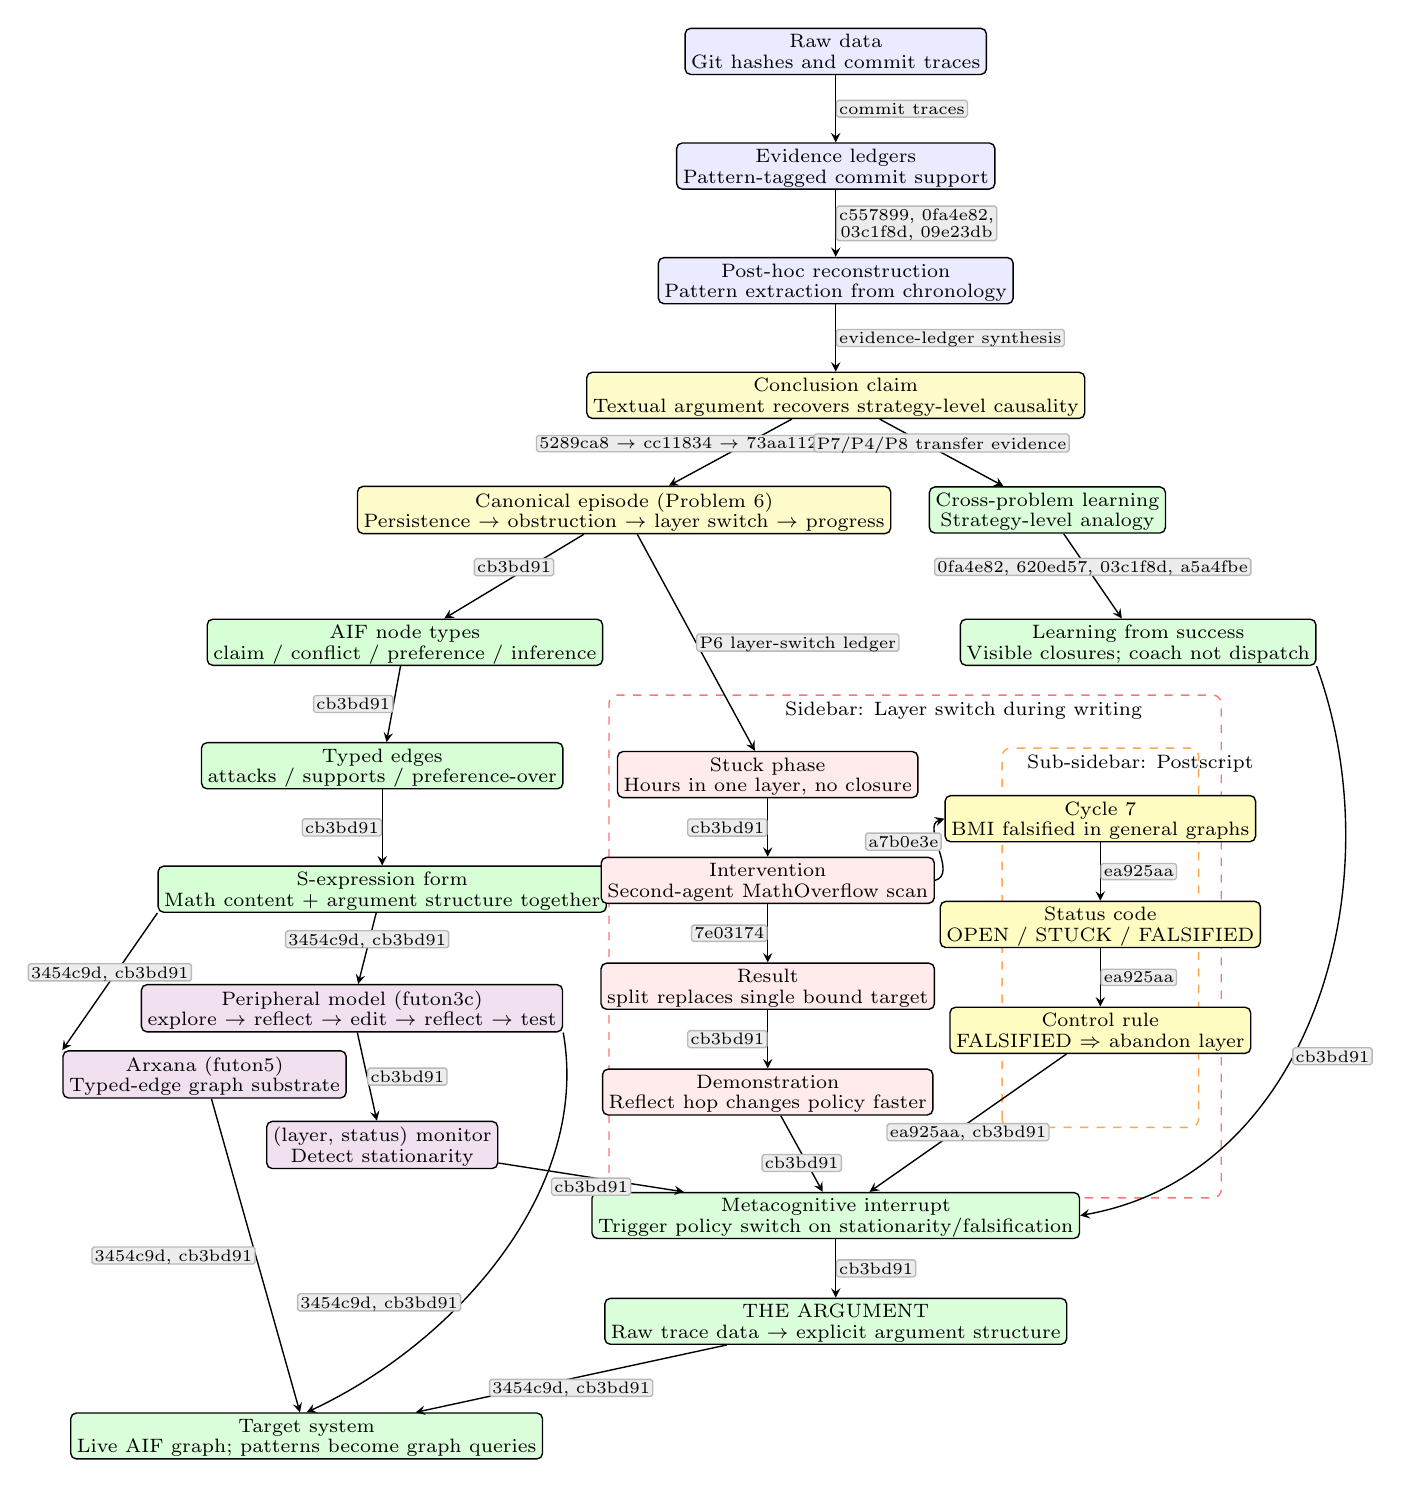
\begin{tikzpicture}[
  x=0.96cm,
  y=1.12cm,
  >=stealth,
  line width=0.5pt,
  text depth=0pt,
  hashlbl/.style={fill=gray!15,draw=gray!55,rounded corners=0.7pt,inner sep=1.0pt,font=\fontsize{5.8}{6.3}\selectfont,align=center},
  box/.style={draw,rounded corners=2pt,align=center,inner sep=2.2pt,font=\fontsize{6.6}{7.4}\selectfont},
  data/.style={box,fill=blue!8},
  synth/.style={box,fill=yellow!20},
  formal/.style={box,fill=green!16},
  infra/.style={box,fill=violet!12},
  side/.style={box,fill=red!8},
  post/.style={box,fill=yellow!24},
  outc/.style={box,fill=green!14}
]

% Top chain
\node[data] (G0) at (0,14.2) {Raw data\\Git hashes and commit traces};
\node[data] (G1) at (0,12.9) {Evidence ledgers\\Pattern-tagged commit support};
\node[data] (G2) at (0,11.6) {Post-hoc reconstruction\\Pattern extraction from chronology};
\node[synth] (C0) at (0,10.3) {Conclusion claim\\Textual argument recovers strategy-level causality};

% Mid layer
\node[synth] (C1) at (-2.8,9.0) {Canonical episode (Problem 6)\\Persistence $\to$ obstruction $\to$ layer switch $\to$ progress};
\node[outc]  (X0) at (2.8,9.0) {Cross-problem learning\\Strategy-level analogy};

% Left formal/infrastructure
\node[formal] (A0) at (-5.7,7.5) {AIF node types\\claim / conflict / preference / inference};
\node[formal] (A1) at (-6.0,6.1) {Typed edges\\attacks / supports / preference-over};
\node[formal] (A2) at (-6.0,4.7) {S-expression form\\Math content + argument structure together};
\node[infra]  (I0) at (-8.35,2.60) {Arxana (futon5)\\Typed-edge graph substrate};
\node[infra]  (I1) at (-6.4,3.35) {Peripheral model (futon3c)\\explore $\to$ reflect $\to$ edit $\to$ reflect $\to$ test};
\node[infra]  (I2) at (-6.0,1.8) {(layer, status) monitor\\Detect stationarity};

% Right learning
\node[outc] (X1) at (4.0,7.5) {Learning from success\\Visible closures; coach not dispatch};

% Sidebar region
\draw[red!55,dashed,rounded corners=3pt] (-3.0,1.2) rectangle (5.1,6.9);
\node[font=\scriptsize,anchor=west] at (-0.8,6.75) {Sidebar: Layer switch during writing};

\node[side] (S0) at (-0.9,6.0) {Stuck phase\\Hours in one layer, no closure};
\node[side] (S1) at (-0.9,4.8) {Intervention\\Second-agent MathOverflow scan};
\node[side] (S2) at (-0.9,3.6) {Result\\split replaces single bound target};
\node[side] (S3) at (-0.9,2.4) {Demonstration\\Reflect hop changes policy faster};

\draw[orange!70,dashed,rounded corners=3pt] (2.2,2.0) rectangle (4.8,6.3);
\node[font=\scriptsize,anchor=west] at (2.4,6.15) {Sub-sidebar: Postscript};
\node[post] (P0) at (3.5,5.5) {Cycle 7\\BMI falsified in general graphs};
\node[post] (P1) at (3.5,4.3) {Status code\\OPEN / STUCK / FALSIFIED};
\node[post] (P2) at (3.5,3.1) {Control rule\\FALSIFIED $\Rightarrow$ abandon layer};

% Bottom
\node[outc] (X2) at (0.0,1.0) {Metacognitive interrupt\\Trigger policy switch on stationarity/falsification};
\node[outc] (T0) at (0.0,-0.2) {THE ARGUMENT\\Raw trace data $\to$ explicit argument structure};
\node[outc] (T1) at (-7.0,-1.5) {Target system\\Live AIF graph; patterns become graph queries};

% Edges and labels
\draw[->] (G0) -- (G1) node[midway,right,hashlbl] {commit traces};
\draw[->] (G1) -- (G2) node[midway,right,hashlbl] {\hash{c557899}, \hash{0fa4e82},\\\hash{03c1f8d}, \hash{09e23db}};
\draw[->] (G2) -- (C0) node[midway,right,hashlbl] {evidence-ledger synthesis};
\draw[->] (C0) -- (C1) node[midway,above,hashlbl] {\hash{5289ca8} $\to$ \hash{cc11834} $\to$ \hash{73aa112} $\to$ \hash{7e03174}};
\draw[->] (C0) -- (X0) node[midway,above,hashlbl] {P7/P4/P8 transfer evidence};

\draw[->] (C1) -- (A0) node[midway,above,hashlbl] {\hash{cb3bd91}};
\draw[->] (A0) -- (A1) node[midway,left,hashlbl] {\hash{cb3bd91}};
\draw[->] (A1) -- (A2) node[midway,left,hashlbl] {\hash{cb3bd91}};
\draw[->] (A2.south west) -- (I0.north west) node[midway,above,hashlbl] {\hash{3454c9d}, \hash{cb3bd91}};
\draw[->] (A2) -- (I1) node[midway,above,hashlbl] {\hash{3454c9d}, \hash{cb3bd91}};
\draw[->] (I1) -- (I2) node[midway,right,hashlbl] {\hash{cb3bd91}};

\draw[->] (C1) -- (S0) node[midway,right,hashlbl] {P6 layer-switch ledger};
\draw[->] (S0) -- (S1) node[midway,left,hashlbl] {\hash{cb3bd91}};
\draw[->] (S1) -- (S2) node[midway,left,hashlbl] {\hash{7e03174}};
\draw[->] (S1.east) to[out=14,in=198] node[pos=0.40,left,yshift=6pt,hashlbl] {\hash{a7b0e3e}} (P0.west);
\draw[->] (S2) -- (S3) node[midway,left,hashlbl] {\hash{cb3bd91}};
\draw[->] (S3) -- (X2) node[midway,below,hashlbl] {\hash{cb3bd91}};

\draw[->] (P0) -- (P1) node[midway,right,hashlbl] {\hash{ea925aa}};
\draw[->] (P1) -- (P2) node[midway,right,hashlbl] {\hash{ea925aa}};
\draw[->] (P2) -- (X2) node[midway,below,hashlbl] {\hash{ea925aa}, \hash{cb3bd91}};

\draw[->] (X0) -- (X1) node[midway,above,hashlbl] {\hash{0fa4e82}, \hash{620ed57}, \hash{03c1f8d}, \hash{a5a4fbe}};
\draw[->] (X1.south east) to[out=-70,in=10] node[pos=0.58,right,hashlbl] {\hash{cb3bd91}} (X2.east);
\draw[->] (I2) -- (X2) node[midway,below,hashlbl] {\hash{cb3bd91}};
\draw[->] (X2) -- (T0) node[midway,right,hashlbl] {\hash{cb3bd91}};
\draw[->] (T0) -- (T1) node[midway,below,hashlbl] {\hash{3454c9d}, \hash{cb3bd91}};
\draw[->] (I0) -- (T1) node[midway,left,hashlbl] {\hash{3454c9d}, \hash{cb3bd91}};
\draw[->] (I1.south east) to[out=-80,in=25,looseness=0.90] node[pos=0.62,left,hashlbl] {\hash{3454c9d}, \hash{cb3bd91}} (T1.north);

\end{tikzpicture}
\endgroup

\caption{The Argument (Conclusion recapitulation): git hashes as raw trace data feed evidence ledgers and post-hoc pattern reconstruction; the conclusion makes this into an explicit argument (AIF node/edge typing, S-expression form, and infrastructure path via Arxana plus peripherals). The sidebar and sub-sidebar episodes are integrated as live evidence for the metacognitive interrupt claim: monitor \((\mathrm{layer},\mathrm{status})\), trigger policy switch on stationarity/falsification, and move from retrospective prose toward real-time argumentative structure.}
\end{figure}
\clearpage

\begin{figure}[p]
\centering
\includegraphics[width=\textwidth,height=0.86\textheight,keepaspectratio]{plates/problem6-a-to-ef-v2.png}
\caption{Problem 6 strategy flow (v2, 9-cycle): from leverage-split dispatch through Neumann/operator-bound attack (C4), BR1--BR4 blocking and threshold relaxation (C5), bridge~B leverage-ordered greedy (C6), BMI falsification (C7), to the Sparse/Strong Dichotomy resolution (C9). Green = proved, yellow = pivot/open, dashed red = falsified. $K_n$ closed with $c_0 = 1/3$; general case conditional on the Strong Dichotomy conjecture (0/148 counterexamples).}
\end{figure}
\clearpage

\begin{figure}[p]
\centering
\includegraphics[width=\textwidth,height=0.86\textheight,keepaspectratio]{plates/problem6-v6.png}
\caption{Problem 6 strategy flow (v6, Cycle~4 focus): operator-bound reduction around the Tur\'an/greedy/pigeonhole core, with Neumann-series amplification controlled via monotonicity and an operator bound for \(\rho_1\). Remaining open node: the trace-gap inequality (\(\alpha < 1/2\), equivalently \(\mathrm{tr}(F) > 2\sum \mu_i(1-\mu_i)/\mu_{\max}\)) needed for full general-graph closure.}
\end{figure}
\clearpage

\begin{figure}[p]
\centering
\includegraphics[angle=90,totalheight=0.86\textheight,keepaspectratio]{plates/problem4-v3.png}
\caption{Problem 4 (v3): finite-free Stam architecture with case decomposition and proof-status stratification.}
\end{figure}
\clearpage

\begin{figure}[p]
\centering
\includegraphics[width=\textwidth,height=0.86\textheight,keepaspectratio]{plates/problem8-v3.png}
\caption{Problem 8 (v3): Lagrangian polyhedral smoothing route with product-smoothing and edge generating-function steps.}
\end{figure}
\clearpage

\begin{figure}[p]
\centering
\includegraphics[width=\textwidth,height=0.86\textheight,keepaspectratio]{plates/problem9-v2.png}
\caption{Problem 9 (v2): rank-1 scaling characterization and polynomial nonvanishing witness flow.}
\end{figure}
\clearpage

\begin{figure}[p]
\centering
\includegraphics[width=\textwidth,height=0.86\textheight,keepaspectratio]{plates/problem10-v2.png}
\caption{Problem 10 (v2): preconditioned-Kronecker solve architecture and complexity path.}
\end{figure}
\clearpage


\backmatter
\begin{thebibliography}{99}

\bibitem{lakatos1976}
I.~Lakatos,
\emph{Proofs and Refutations: The Logic of Mathematical Discovery},
Cambridge University Press, 1976.

\bibitem{pease2017}
A.~Pease, J.~Lawrence, K.~Budzynska, J.~Corneli, and C.~Reed,
``Lakatos-style collaborative mathematics through dialectical,
structured and abstract argumentation,''
\emph{Artificial Intelligence} \textbf{246} (2017), 181--219.

\bibitem{corneli2017}
J.~Corneli, U.~Martin, D.~Murray-Rust, and A.~Pease,
``Towards mathematical AI via a model of the content and process of
mathematical question and answer dialogues,''
in \emph{Proc.\ CICM 2017}, Springer LNCS, 2017.

\bibitem{corneli2013}
J.~Corneli,
\emph{Peer Produced Peer Learning: A Mathematics Case Study},
PhD thesis, The Open University, 2014.

\bibitem{fowler2012}
J.~Fowler,
``Finiteness properties of rational Poincar\'e duality groups,''
\texttt{arXiv:1204.4667}, 2012.

\bibitem{bartels2014}
A.~Bartels, F.\,T.~Farrell, and W.~L\"uck,
``The Farrell--Jones conjecture for cocompact lattices in virtually
connected Lie groups,''
\emph{J.~Amer.\ Math.\ Soc.} \textbf{27} (2014), 339--388;
\texttt{arXiv:1101.0469}.

\bibitem{hughesWeinberger2001}
B.~Hughes and S.~Weinberger,
``Surgery and stratified spaces,''
in \emph{Surveys on Surgery Theory}, Vol.~2,
Ann.\ of Math.\ Studies 149, 2001;
\texttt{arXiv:math/9807156}.

\bibitem{lopezdeMedrano1971}
S.~L\'opez de Medrano,
\emph{Involutions on Manifolds},
Ergebnisse der Mathematik \textbf{73}, Springer, 1971.

\bibitem{ranicki1998}
A.~Ranicki,
\emph{High-Dimensional Knot Theory: Algebraic Surgery in Codimension~2},
Springer Monographs in Mathematics, 1998.

\bibitem{wall1999}
C.\,T.\,C.~Wall,
\emph{Surgery on Compact Manifolds},
2nd ed., Mathematical Surveys and Monographs \textbf{69}, AMS, 1999.

\end{thebibliography}

\end{document}
